% This file should be replaced with your file with an thesis content.
%=========================================================================
% Authors: Michal Bidlo, Bohuslav Křena, Jaroslav Dytrych, Petr Veigend and Adam Herout 2019

% For compilation piecewise (see projekt.tex), it is necessary to uncomment it and change
% \documentclass[../projekt.tex]{subfiles}
% \begin{document}

\chapter{Introduction}
% Finite Automata + Mata

Finite automata can be found in numerous fields both in research and in practice.
There are several automata libraries, each with their own set of supported automata types and operations.
Their respective design decisions gives various advantages and disadvantages for each library.
Recently, a new finite automata library, called \mata, emerged.
\mata aims to remain simple, yet perform very fast for a large set of automata operations commonly used in various applications such as string constraints solving, reasoning about regular expressions, regular model checking, or in decision procedures for logics such as WS1S or quantified Presburger arithmetic.

Efficiency of automata algorithms used in these fields is crutial since problems from all of these fields are computationally hard.
Many automata libraries are well-optimized on only one subset of operations, or presume a certain general approach to using them.
\mata points at fast computation of operations in various frameworks, providing optimized general operations on finite automata as well as several purpose-specific algorithms used in specific fields.

\mata's underlying data structures are designed in such a way that they provide sufficient performance, but also enable easy modification by the user for their own uses and extensible framework for adding new automata types, purpose-specific operations, or additional maintanence of related context while keeping the existing infrastructure working with as minimal number of changes required as possible.

In this work, we intend on utilizing the extensibility of \mata and its underlying data structures to add support for finite state transducers while maintaining the main ideas of \mata: being fast, and easy to extend or modify.

% Finite Transducers
Finite transducers are finite-state machines.
They are similar to finite automata, but finite transducers work with multiple memory tapes.
Each tape represents a regular language where finite transducers performs mapping between these languages, and, more preciselly, between words in each language.
Finite transducers model relations (called \emph{rational relations}) between regular languages.
Heneforth, each finite transducer can be thought of as a translator translating (transducing) between the languages (a 2-tape finite transducer precisely models a translator from an input language to a output language, modelling a so-called \emph{binary rational relation}).
In this work, we usually work with binary rational relations, but in general an \emph{n-ary rational relation} can be modelled by a n-tape transducer.

% String Solving + Noodler
In the recent decades, we have seen a rapid growth of  various procedures for SMT string solving, implemented in numerous state-of-the-art SMT solvers.
The importance of efficient algorithms for deciding satisfiability of SMT formulae is underlined by everyday applications in the industry such as AWS~\cite{Rungta2022} or the ongoing anual competion SMT-COMP~\cite{smt_comp}.

Recent advances in analysis of programs manipulating strings, string solving, automatically solving string constraints over string languages, have heightened the importance of modelling string replacement operations.
Such operations allow for replacing a substring specified by a regular langauge with another string.
The appliations are widely used in web applications such as implicit browser transductions, or replace functions such as \emph{replace} and \emph{replace-all} functions.
One of the most important applications of string-replace operations is defense against attacks such as cross-site scripting or code injection in web applications.
Untrusted inputs from a user are to be sanitized (e.g. by escaping the input string) in order to prevent arbitrary malicious code execution.
We need a toolset to verify that such sanitizations are correct and safe.
SMT solver with support for replace operations can be used to decide this.

Another applications are implicit browser transductions.
HTML codes need to be coded and decoded in the input strings (replacing \texttt{\&\#39;} by a single quote \texttt{'}).
% Application of transducers for string solving
Finite transducers are ideal for modelling both the sanitization operations as well as the implicit browser transductions:
Both these applications create relations between two languages, mapping strings from one language to the other which can be modelled by finite transducers.
Finite transducers can model implicit browser transductions directly.
They can be used to model string-replace operations for sanitization operations and the resulting replacement (the generated language) can be tested for emptiness of intersection with the typical cross-site scripting attack patterns database, represented as a regular languages.
Such constraints are presented to an SMT solver to decide its satisfiability.

We have introduced a new SMT string solver \noodler which utilizes an automata-based approach to string solving with finite automata and operations on them implemented in \mata as the backbone of the whole decision procedure of \noodler.

\paragraph{Contribution.}
In this work, we study automata models called finite transducers and their applicability to string solving. We implement the proposed solution in \mata and evaluate the implemented solution on variety of benchmark problems from practice.

Namely, the constributions of this work can be summarized as follows:
\begin{itemize}
  \item Design of data structures and algorithms for finite transducers with regard to existing and planned data structures and algorithms in \mata.
  \item Implementation of the proposed data structures and algorithms in automata library \mata,
  \item A new benchmark of replace operations encoded as finite transducers derived from SMT-LIB benchmarks with replace operations. The operations in the benchmark performed are the typically used operations in string solving on real problems, and
  \item Experimental evaluation of the implemented algorithms on a variety of benchmark problems from practice.
\end{itemize}

\chapter{Preliminaries}
In this chapter, we will define several terms and notions used throughout this thesis.
We follow the usual definitions of automata theory, as used in works such as~\cite{Esparza} or~\cite{Sipser} with custom modifications and additions.

\paragraph{Alphabets.}
We define an \emph{alphabet} $\Sigma = \{ a, b, c, \ldots \}$ as a set of \emph{symbols} where
symbols are usually denoted by $a, b, c, \ldots$.
$\Sigma^*$ denotes a set of all finite \emph{words} (or \emph{strings}) over the alphabet $\Sigma$.
Furthermore, we use two special symbols: an \emph{epsilon symbol} $\eps \notin \Sigma$, representing an empty symbol (or word, $\eps \in \Sigma^*$), and a \emph{don't care symbol}, denoted $\dontCare$, representing any single symbol from $\Sigma$.
\emph{Alphabet with epsilon symbols} (epsilons) is denoted $\SigmaEps = \Sigma \cup \{ \eps \}$.

We denote \emph{concatenation} on words $w_1$, $w_2$ using $w_1 \concat w_2$, sometimes for convenience omitting the concatention operator $w_1w_2$, where $\eps$ is the neutral element of concatenation ($\eps \concat w_1 = w_1 \cdot \eps = w_1$).

\section{Finite Automata}

In this section, we lay foundation to finite automata and their aspects which are utilized in this work.

\paragraph{Nondeterministic finite automata.}
A \emph{nondeterministic finite automaton} (\emph{NFA}) over the alphabet $\Sigma$ is a 5-tuple $\aut = (\states, \Sigma, \post, \initialStates, \finalStates)$ where
\begin{itemize}
    \item $\states$ is a finite set of \emph{states},
    \item $\Sigma$ is the alphabet of $\aut$,
    \item $\post: \states \times \Sigma \rightarrow 2^{\states}$ is a \emph{symbol-post function} where $\move{q}{a}{q'}$ (or $(q, a, q')$) for $q' \in \post(q, a)$ is a \emph{transition},
    \item $\initialStates \subseteq \states$ is a finite set of \emph{initial states}, and
    \item $\finalStates \subseteq \states$ is a finite set of \emph{final states}.
\end{itemize}

A set of all transitions of $\aut$ forms a transition relation of $\aut$, denoted $\Delta$. $\Delta(q, a) \equiv \post(q, a)$.

Furthermore, we define a \emph{state-post function} $\post(q) = \{ (a, \post(q, a)) \mid \post(q, a) \neq \emptyset \}$ for a state $q$.
Symbol-post function and State-post function are called \emph{post-image functions}.
$\post$ can be generalized to a set of source states over a given transtision symbol, $\post(S, a)$ where $S \in \states$ and $a \in \Sigma$ as $\post(S, a) = \bigcup_{s \in S} \post(s, a)$.


An \emph{NFA with epsilon symbols} is a 5-tuple $\aut = (\states, \SigmaEps, \post, \initialStates, \finalStates)$ where
\begin{itemize}
    \item $\states$, $\initialStates$, $\finalStates$ are the same as for normal NFA, and
    \item symbol-post function $\post: \states \times \SigmaEps \rightarrow 2^{\states}$ allows epsilon symbols.
\end{itemize}
We will often denote NFA with epsilons as just NFA where it is clear whether we allow epsilon transitions or not in regard to the context.

We define a \emph{run} (\emph{path}) of $\aut$ over a word $w \in \Sigma^*$ as a sequence of states and symbols $q_0a_1q_1a_2\ldots a_nq_n$ where $\forall 1 \leq i \leq n: q_i \in \post(q_{i-1}, a_i) \land a_i \in \SigmaEps \land w = a_1a_2\ldots a_n$.
We further distinguish runs as \emph{accepting runs} and \emph{nonaccepting runs} (\emph{not accepting runs}).
A run is accepting if and only if $q_0 \in \initialStates  o$ and $q_n \in \finalStates$.
A (potentially infinite) set of words for which there exists an accepting run of $\aut$ defines a regular language $\langof{\aut} \subseteq \SigmaEps$ of NFA $\aut$.

States $\states$ can be divided into \emph{useful states} and \emph{useless} states.
A state $q$ is useful if there exists an accepting run over states $q_0, q_1, \ldots, q_n$ where $q \in \{ q_0, q_1, \ldots, q_n \}$.
Otherwise, $q$ is useless.

We also distinguish between \emph{reachable} and \emph{unreachable} states.
A state $q$ is reachable if there exists a path $q_0a_1, \ldots, a_nq$ in $\aut$ such that $q_0 \in \initialStates$.

% An NFA where all $q \in \states$ are useful is called to be \emph{trimmed}.

\paragraph{Deterministic finite automata.}
We call an NFA $\aut = (\states, \Sigma
% \SigmaEps
, \post, \initialStates, \finalStates)$ a \emph{deterministic finite automaton} (\emph{DFA}) iff $\forall q \in \states, a \in \Sigma: |\post(q, a)| \leq 1
% \land |\post(q, \eps)| = 0
$, and $|\initialStates| = 1$.

\begin{definition}[\textbf{Powerset (\textbf{subset}) construction}] \hfill \newline
    The algorithm of powerset (subset) construction creates deterministic finite automaton from its equivalent non-deterministic finite automaton. Powerset construction produces a \dfa $A'$, where $\states' = 2^\states$, $\finalStates' = \{S \in \states' | S \cap \finalStates \neq \emptyset\}$, $\initialStates' = \initialStates$ and for $S \in \states': \post'(S, a) = \bigcup_{s \in S} \post(s, a)$.
\end{definition}

\begin{definition}[\textbf{Product construction}] \hfill \newline
Product construction is an algorithm where, given two \nfas $A_1 = (\states_1, \Sigma, \post_1, \initialStates_1, \finalStates_1)$ and $A_2 = (\states_2, \Sigma, \post_2, \initialStates_2, \finalStates_2)$ over an alphabet $\Sigma$, the algorithm yields a product \nfa $A$ as a 5-tuple deterministic finite automaton $A = (\states, \Sigma, \post, \initialStates, \finalStates)$ where:
\begin{itemize}
    \item $\states = \states_1 \times \states_2$,
    \item $\post: \states \times \Sigma \rightarrow{} P(\states)$,
    \item $\initialStates = \initialStates_1 \times \initialStates_2$, and
    \item $\finalStates = \finalStates_1 \times \finalStates_2$.
\end{itemize}
\end{definition}

$\post$ is constructed as $([q_1, q_2], a) = \post_1(q_1, a) \times \post_2(q_2, a)$ where $[q_1, q_2]$ denotes a pair of states, often called \emph{macrostate} or \emph{product state}. For pairs of states $q_1 \in \states_1$ and $q_2 \in \states_2$ and a common transition symbol $a$ of transitions $q'_1 \in \post_1(q_1, a)$ and $q'_2 \in \post_2(q_2,a)$, a single product transition is denoted as $[q_1, q_2] \xrightarrow{a} [q'_1, q'_2]$, where $[q'_1, q'_2] \in \post([q_1, q_2], a)$ for the corresponding states $[q_1, q_2]$ and $[q'_1, q'_2]$ in $A$.

When applied for computing an \emph{intersection} of \nfas, the language of $A$ is equal to $ \langof{A} = \langof{A_1} \cap \langof{A_2} $.

In this work, we will utilize the classic product construction algorithm, as shown in Algorithm~\ref{productConstructionAlg}.

\begin{algorithm}[ht]
\caption{Product construction algorithm in its classic implementation.}\label{productConstructionAlg}
\SetKwData{Left}{left}\SetKwData{This}{this}\SetKwData{Up}{up}
\SetKwFunction{Union}{Union}\SetKwFunction{FindCompress}{FindCompress}
\SetKwInOut{Input}{Input}\SetKwInOut{Output}{Output}
\DontPrintSemicolon
\Input{ NFA $A_1 = (\states_1, \Sigma, \post_1, \initialStates_1, \finalStates_1)$, NFA $A_2 = (Q_2, \Sigma, \post_2, \initialStates_2, \finalStates_2)$}
\Output{ NFA $A = (A_1 \cap A_2) = (\states, \Sigma, \post, \initialStates, \finalStates)$ with $\langof{A_1 \cap A_2} = \langof{A_1} \cap \langof{A_2}$}
\BlankLine
$\states, \post, \finalStates \gets \emptyset$ \\
$\initialStates \gets \initialStates_1 \times \finalStates_2$ \\
$W \gets  I$

\While{$W \neq \emptyset$}{
    \textbf{pick} $[q_1, q_2]$ \textbf{from} $W$ \\
    \textbf{add} $[q_1, q_2]$ \textbf{to} $\states$ \\
    \If{$q_1 \in \finalStates_1$ and $q_2 \in \finalStates_2$} {
        \textbf{add} $[q_1, q_2]$ \textbf{to} $\finalStates$
    }
    \ForAll{$a \in \Sigma$}{
        \ForAll{$q'_1 \in \post_1(q_1, a), q'_2 \in \post_2(q_2, a)$}{
            \If{$[q'_1, q'_2] \notin Q$}{\textbf{add} $[q'_1, q'_2]$ \textbf{to} $W$}
            \textbf{add} $[q'_1, q'_2] \textbf{ to } \post([q_1, q_2], a)$
        }
    }
}
\end{algorithm}

\section{Finite State Transducers}

In this section, we define finite state transducers and corresponding operations.


\paragraph{Nondeterministic finite state transducers.}
An $n$-tape \emph{nondeterministic finite state transducer} (\emph{NFST}; \emph{nondeterministic finite transducer}, \emph{NFT}) over an alphabet $\Gamma$ is a 5-tuple $\transducer = (\states, \Gamma, \post, \initialStates, \finalStates)$ where
\begin{itemize}
    \item $\states$ is a finite set of \emph{states},
    \item $\Gamma = (\SigmaEps)^n$ is an $n$-tape alphabet of $\transducer$.
    \item $\post: \states \times \Gamma \rightarrow 2^{\states}$ is a \emph{symbol-post function} where $\move{q}{\gamma}{q'}$ (or $(q, \gamma, q')$) for $q' \in \post(q, \gamma)$ is a \emph{transition} for $\gamma = \begin{bsmallmatrix} a^1 & a^2 & \ldots & a^n\end{bsmallmatrix} = (a^1, a^2, \ldots, a^n) \in (\SigmaEps)^n$,
    \item $\initialStates \subseteq \states$ is a finite set of \emph{initial states}, and
    \item $\finalStates \subseteq \states$ is a finite set of \emph{final states}.
\end{itemize}

\nft $\transducer$ is syntactically an NFA over $\Gamma$.
$\transducer$ accepts word $\transWord{w} = \gamma_1 \circ \gamma_2 \circ \ldots \circ \gamma_m = (a^1_1, a^2_1, \ldots, a^n_1) \circ (a^1_2, a^2_2, \ldots, a^n_2) \circ \ldots \circ (a^1_m, a^2_m, \ldots, a^n_m) $ if there exists an accepting run of $\transducer$ for $\transWord{w}$ where $\circ$ is a concatenation operator performing component-wise concatenation over tuples: $(a^1_1, a^2_1, \ldots, a^n_1) \circ (a^1_2, a^2_2, \ldots, a^n_2) = (a^1_1a^1_2, a^2_1a^2_2, \ldots, a^n_1a^n_2)$.
When the context is clear, we sometimes omit $\circ$, similarly as for NFA.

A (potentially infinite) set of words for which there exists an accepting run of $\transducer$ defines a \emph{rational relation} $\relationof{\transducer} \subseteq (\SigmaEps^*)^n$ of \nft $\transducer$.

\paragraph{Deterministic finite transducers.}
An $n$-tape \emph{deterministic finite state transducer} (\emph{DFST}; \emph{deterministic finite transducer}, \emph{DFT}) over an alphabet $\Gamma$ is a 5-tuple $\transducer = (\states, \Gamma, \post, \initialStates, \finalStates)$ where all elements in the tuple are the same as for \nft, except for the definition of $\post$ where
\begin{itemize}
    \item $\post: \states \times \Gamma \rightarrow \states$ is a \emph{symbol-post function} where $\move{q}{\gamma}{q'}$ (or $(q, \gamma, q')$) for $q' = \post(q, \gamma)$ is a \emph{transition} for $\gamma = \begin{bsmallmatrix} a^1 & a^2 & \ldots & a^n\end{bsmallmatrix} = (a^1, a^2, \ldots, a^n) \in (\SigmaEps)^n$. That is, $|\post(q, \gamma)| \leq 1$, and
    \item $|\initialStates| = 1$.
\end{itemize}

% TODO: Synchronized transducer and synchronized rational language + its properties?

In this work, we will often limit ourselves to 2-tape \nfts (\dfts), called \emph{((non)deterministic) finite state input output transducers} where the first tape is the \emph{input tape} and the second tape is the \emph{output tape}.

Unless we explicitly state the number of tapes, we will further consider 2-tape \nfts.

% TODO: Input, output projection.
% TODO: Composition, Application.






\chapter{Theoretical Background}
\section{Finite Automata}
\subsection{Mata}

\mata is a new finite automata library, built with simplicity, extensibility and performance in mind.
\mata currently supports only (non)deterministic finite automata.

The performance of \mata have been evaluated in~\cite{cade23_reasoning_regular_properties_comparision_DBLP:conf/cade/FiedorHHRSV23} (as \enfa), \cite{tacas24_mata_10.1007/978-3-031-57249-4_7}.
Furthermore, \mata is used as an underlying finite automata library for a novel string solver \noodler in~\cite{fm23fm23_equations_synergy_regular_constraints_DBLP:conf/fm/BlahoudekCCHHLS23, oopsla23_stabilization_DBLP:journals/pacmpl/ChenCHHLS23,tacas24_noodler_10.1007/978-3-031-57246-3_2}, where \mata handles creation and storing of finite automata and performing automata operations on them.

In all of these papers, \mata performs well, and outperforms even the state-of-the-art automata libraries such as \automatajar, \awali, \vata, \brics, \automatanet, \automatapy, \fado.~\cite{tacas24_mata_10.1007/978-3-031-57249-4_7}.

From these results, we can see that \mata offers an interesting set of features, namely performance and extensibility, and is applicable in numerous areas of both research and practical use-cases.

To further extend the applicability of \mata in string solving, abstract regular model checking, reasoning about regular expressions, etc., adding support for other finite automata types is planned.
One of such automata are finite transducers.
Other types include binary decision diagrams (BDDs), finite automata with registers for counting operations, or arbitrary registers.


% $\Delta$ stores in memory only those state-posts (a, post(q, a)) where
% \mid \post(q, a) \neq \emptyset

% Mona?
\section{Finite Transducers}

\section{String Solving}

During the last two decades, a great development efforts have been put on improving SMT solvers for specific theories (specific constraint languages).
Namely, modelling and deciding constraints over a language of strings, also known as \emph{string solving}, is one of the dominant fields of active research.

The advances in string solving are supported by the application of string solvers (SMT solvers supporting solving constraints over the language of strings) in web services to prevent cross-site scripting or code execution attacks by discovering security vulnerabilities in web applications and web service APIs, as presented by works:~\cite{String_constraints_with_concatenation_and_transducers_solved_efficiently, Composing_Static_and_Dynamic_Analysis_to_Validate_Sanitization_in_Web_Applications, Satisfiability_Modulo_Theories_Introduction_and_Applications, Simple_linear_string_constraints,Z3-str_a_z3-based_string_solver_for_web_application_analysis,S3_A_Symbolic_String_Solver_for_Vulnerability_Detection_in_Web_Applications} and many more.

String solving is especially useful for analysis of security vulnerabilities related to sanitization of text inputs from users on websites.
This prevents crackers from injecting malicious code into the website and spreading the code between the users of said website using techniques such as cross-site scripting: executing arbitrary malicious code on the user's local browser environment.
Sanitization of text inputs is one of many use-cases where finite transducers can be utilized.

\paragraph{Cross-site scripting attack.}
Take a look at one textbook example of a cross-site scripting attack where text inputs are sanitized incorrectly in Listing~\ref{listing:not_sanitized_example}, allowing for insertion of malicious script executing arbitrary code.
\begin{listing}[!ht]
\caption{Example of an cross-site scripting attack where an incorrectly sanitized user input can be stored directly the database.}
\label{listing:not_sanitized_example}
\begin{minted}
[
  linenos
]{php}
  <?php
    $input_from_user = $_POST["update_account_form"];
    $body = replace(
      "/\<script.*?\>.*?\<\/script.*?\>/i",
      "",
      $input_from_user);
    update_user_account($body);
  ?>
\end{minted}
\end{listing}

The example accepts input from a user who fills in a form to update user account information on the website.
The input is taken through a sanitization function \texttt{replace} which replaces a substring matched by the regular expression in the first argument by the string in the second argument in the string suplied by its last argument.
The idea is that all occurrences of malicious scripts inside \texttt{<script>} and \texttt{</script>} tags are replaced with an empty string.

However, this sanitization function may be incorrect.
Depending on the replace semantics, the replacement of \texttt{.*} (Kleene star) can be performed either greedily (at which point the function would sanitize correctly) or reluctantly (the function would sanitize incorrectly).
Let us see an example of cracker's input:
\begin{center}
 \texttt{<<script></script>script>perform\_malicious\_action("danger")</script>}
\end{center}
which will be replaced with the reluctant semantics to
\begin{center}
 \texttt{<script>perform\_malicious\_action("danger")</script>}
\end{center}

matching only the inner pair of \texttt{<script>}, \texttt{</script>} tags.

But if we apply greedy semantics, the user input will be correctly sanitized:
\begin{center}
 \texttt{""}
\end{center}
where cross-site scripting is prevented from occuring.

A different example~\ref{listing:not_sanitized_implicit_browser_transductions_example} shows how incorrectly handled implicit browser transductions in JavaScript can allow for cross-site scripting attack by executing arbitrary malicious code on the user's local browser.
Having an input from a user (stored in variable \texttt{goal}), we want to show a button with the goal specified by the user which executes the corresponding action. Ideally, \texttt{performAction(goal)} function would refuse to execute the action if the action was unspecified (therefore possibly malicious).
If we pass some valid string as a user, for example \texttt{Study \& Research}, the implicit browser transductions correctly handle the input, encode \texttt{\&} and the button is displayed.
However, if an attacker passes a string that contains an arbitrary malicious code, constructed in such a way that escaping the input will produce an executable piece of code instead of a button, the browser can perform an action specified by the attacker (here simple \texttt{alert(danger)}) on user's browser.

\begin{listing}[!ht]
\caption{Example of an cross-site scripting attack using incorrectly handled implicit browser transductions where a malicious attacker's input can be run directly in the user's local browser.}
\label{listing:not_sanitized_implicit_browser_transductions_example}

    \begin{minted}{javascript}
var text = htmlEscape(goal);
var action = escapeString(text);
element.innerHTML = '<button onclick=
"performAction(\'' + action + '\')">' + text + '</button>';
    \end{minted}

    \begin{minted}{javascript}
<button onclick="performAction('Study &amp; Research')">
  Study &amp; Research</button>
    \end{minted}

    \begin{minted}{javascript}
<button onclick="performAction('&#39;);alert(danger);//')">
  &#39;);alert(1);//')</button>
    \end{minted}
\end{listing}

Sadly, such examples does not occur only in textbooks. Real websites use sanitization functions sparingly or do not sanitize user inputs at all.

SMT solvers with support for finite transducers can implement such sanitization functions where finite transducers are used for modelling the rewriting rules~\cite{rewriting_rules_kaplan94, rewriting_rules_karttunen97}.
However, as we have seen in the example above, choosing the correct replacement semantics is important as well.
Finite transducers can directly implement both the reluctant replacement and greedy replacement.
Depending on the use-case, both semantics can be useful.
Such SMT solver with finite transducers can be then used for automatic discovery of cross-site scripting vulnerabilities in source code as well as real-time sanitization.

\subsection{Noodler}

An SMT string solver called \noodler~\cite{fm23_equations_synergy_regular_constraints_DBLP:conf/fm/BlahoudekCCHHLS23, oopsla23_stabilization_DBLP:journals/pacmpl/ChenCHHLS23,tacas24_noodler_10.1007/978-3-031-57246-3_2}, using \mata as the underlying automata library, is a new addition to the set of SMT solvers solving string constraints.
\noodler is based on \ziii~\cite{z3} where it replaces its theory of string.

\noodler brings a novel approach to solving string constraints using a method called \emph{stabilization}, a new procedure for solving word (dis)equations in combination with regular constraints.

This stabilization-based procedure is seamlessly used in \noodler in combination with the well-used existing algorithms such as
Align\& Split (first implemented in a string solver \norn~\cite{Norn,AutomataSplitting}, and later adopted by a multitude of other state-of-the-art string solvers---\ostrich~\cite{AnthonyTowards2016,AnthonyReplaceAll2018,AnthonyComplex2019,AnthonyRegex2022,AnthonyInteger2020},
\ziiistriiire~\cite{Z3str3RE,BerzishDGKMMN23}, \sloth~\cite{holik_string_2018}, \ldots
), used for converting regular constraints into length constraints, and
Nielsen transformation~\cite{nielsen1917}, used for solving quadratic equations.

Thanks to this combination of approaches, \noodler is able to uniquely utilize information from both the regular constraints and word equations to efficiently prune the searched state space, mitigating the effects of possible combinatorial state space explosion.
This feature of the stabilization-based procedure makes \noodler superior to other state-of-the-art string solvers on many benchmarks, as seen in the latest results from \noodler~\cite{tacas24_noodler_10.1007/978-3-031-57246-3_2}, and in previous articles~\cite{fm23_equations_synergy_regular_constraints_DBLP:conf/fm/BlahoudekCCHHLS23, oopsla23_stabilization_DBLP:journals/pacmpl/ChenCHHLS23}.

\noodler, as opposed to all other state-of-the-art SMT string solvers (with the exception of \ostrich) utilizes finite automata as the underlying data structures to intuitively encode regular constraints.
This gives \noodler unique oportunities for efficient string solving of SMT formulae which other SMT solvers cannot utilize.
Using finite automata models as much as possible allows us to solve the satisfiability of the SMT formula by performing standard automata operations on finite automata representing regular languages of string variables in the formula and corresponding constraints.
The performance results of \noodler clearly show that, when implemented correctly, automata-based algorithms can be more performant than the classic approaches to string solving.
This is the reason why it is so important that all implemented automata models in \mata are as performant as possible.

The only unsupported operations in \noodler are at the time of writing string operations \texttt{str.replace\_all} and \texttt{str.replace\_re\_all} from the theory of strings in SMTLIB~\cite{smtlib_theory_strings}.
Furthermore, the string operations \texttt{str.replace} and \texttt{str.replace\_re} are handled by a modified \noodler version of theory rewriter (replacing \ziii own theory rewriter) applying rewriting rules to convert both operations to a combination of word equations, disequations, and length and regular constraints.
However, the generated corresponding (dis)equations and constraints negatively impact the performance of the overall procedure.

All of these operations can be easily encoded as finite transducers (with the model being implemented in \mata together with the corresponding operations on finite transducers), and resolved by applying standard finite transducer operations on the computed inputs.
For this reason, adding support for finite transducers in \mata is paramount to the capabilities of \noodler and its overall performance.

\chapter{Finite Transducers}

This chapter describes our proposed solution for representation of \nfts in \mata. We describe how we model \nfts in \mata, what data structures we use, how we implement the neessary algorithms working with these data structures.

\begin{example}\label{example:2_tape_nft}
In Figure~\ref{fig:2_tape_nft}, we show a 2-tape input/output \nft accepting a rational relation with an input language of $(abc)^*$ and the corresponding output language where each input transition symbol $a$ is replaced with $bc$, input transition symbol $b$ is erased, and input transition symbol $c$ is replaced with $a$.

\begin{figure}[!ht]
  \centering
  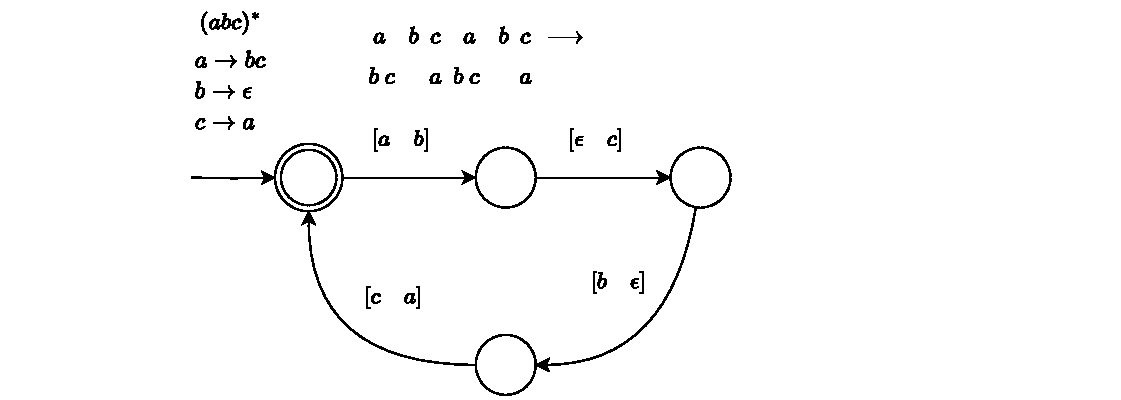
\includegraphics[scale=1.0, keepaspectratio]{obrazky-figures/transducer.drawio.pdf}
  \caption{
    Example of a 2-tape input/output \nft.
  }\label{fig:2_tape_nft}
\end{figure}

\end{example}

\section{Data Structure}
We propose utilizing the existing data structures in \mata (used for NFAs) for implementing finite transducers in \mata.
The main advantage is that NFAs, \nfts, and BDDs can all be implemented using the same single data structure, utilizing a lot of the existing algorithms on the data structures.

\mata provides a base class \nfaClass which encompasses both deterministic and non-deterministic finite automata and operations on them.
Class \nfaClass is a base class from which \nfts, BDDs, and register automata can inherit, including all operations on \nfaClass where only a few specific operations need to be modified for each respective type of finite-state machine.
This hierarchy also allows us to add model-specific operations to each type of automata without modifying operations for the other automata.
BDDs in our representation only extend the functionality of \nfts, and can therefore inherit most of the algorithms from \nfts and only modify some of the algorithms for BDD-specific use-cases.

\begin{figure}[ht]
  \centering
  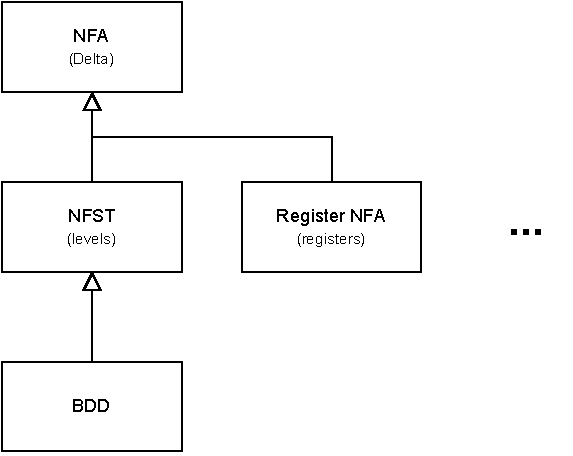
\includegraphics[scale=0.8, keepaspectratio]{jumps_synchronization-NFAs-NFSTs-BDDs-hierarchy.drawio.pdf}
  \caption{
    An inheritance hierarchy for NFAs, \nfts, BDDs, and register automata.
    All of these finite-state machines utilize the same data structure, with mostly the same algorithms where only a few algorithms needs to be modified for each respective type of finite-state machine.
    Each type of finite-state machine can further extend the set of operations by their own specific operations.
    Since BDDs only extend the functionality of transducers, BDDs can inherit directly from \nfts, modifying a few algorithms of \nfts together with the base \nfaClass algorithms.
  }
\end{figure}

Class \nfaClass defines which states in the represented automaton are initial (a set of initial states) and which are final (a set of final states).
Furthermore, \nfaClass allows for storing of arbitraty context in the automaton itself.

The most important data structure for the representation of the finite-state machines and the efficiency of the algorithms run on the representation is the representation of transition relation, called \deltastruct in \mata.
\deltastruct defines the set of states of the finite automaton, and gives the transition relation of the finite automaton.
\deltastruct is designed in such a way that often used operations such as iteration over transitions, adding and removing transitions, are performant, while less often used operations such as reversal of transition relation can be less performant.

States are in \mata represented as unsigned integers, numbered from 0.
This allows adding new states to the automaton to be as easy as getting the number of states in \deltastruct (constant time operation) and adding a number equal to the number of new states we want to add.
Such states are immediatelly allocated in \deltastruct and can be used in initial of final states sets.

Transition symbols are internally stored as unsigned integers as well, numbered from 0, where the last several unsigned integer values are reserved for epsilon symbols.
\mata provides several alphabet types which map the actual transition symbols to their internal values.

The use of unsigned integers for states and symbols gives implicit ordering over both states and symbols and querying them by accessing index corresponding to the internal state/symbol value in an ordered vector.
\deltastruct is a three-level data structure where each level represents one element from the three-tuple $(q, s, q')$ representing a single transition as:
\begin{enumerate}
    \item source states,
    \item transition symbols,
    \item target states.
\end{enumerate}

Each level is internally stored in memory as a sorted vector of unsigned integers, stored in a low-level data structure provided by \mata called \ordvector, a wrapper over \texttt{std::vector} maintaining a set of elements inserted to \texttt{std::vector} ordered.

\ordvector therefore has constant time access to stored elements, operations on the largest element (implemented internally as \texttt{push\_back()}, \texttt{pop\_back()}), fast linear iteration over the elements, and linear union, intersection, and difference.
Since vectors are ordered, lookup for states and symbols is logarithmic using binary search.
Insertion and removal of are logarithmic, but they must shift elements in the memory in the underlying \texttt{std::vector} which slows the operations down.

Due to this, \mata tries to iterate over \ordvector as often as possible since internally, \texttt{std::vector} stores elements in a continuous array on heap with good memory locality, and add elements one after the other in an ascending order given by the value of the inserted elements at the end of the ordered vector.
Several algorithms such as synchronized traversal over multiple ordered vectors.
General insertion and removal of transitions are logarithmic, but \mata algorithms are written in such a way that the general insertion and removal are seldom used.

This pairs well with underlying data structures for sets of initial and final states, implemented as sparse sets~\cite{sparseset93} allowing for constant element lookup, insertion and removal, and fast linear iteration through elements.

The Figure~\ref{fig:delta_struct} visualizes the three-level \deltastruct data structure. We can see that the when we access by source state $q$ the index in the first vector of source states, we get a vector post of type \statepost (\statepost[q]), representing $\post(q)$, which is a vector of symbol posts for each transition symbol $a$ leading from source state $q$, of type \symbolpost.
Each symbol post for symbol $a$ represents $\post(q, a)$, storing the transition symbol $a$ and a set of target states represented as a \ordvector.

% {\tiny
\begin{figure}[ht]
\begin{center}
% \includegraphics[width=10cm]{images/Delta.pdf}
% TODO: Replace with my own image of Delta struct.
\definecolor{color1}{RGB}{54,174,124}
\definecolor{color2}{RGB}{24,116,152}
\begin{tikzpicture}[
    circ/.style={draw,circle,inner sep=0pt,minimum size=2pt,fill},
    arr/.style={->,thick,>=stealth},
    type/.style={color2,dashed,thick},
    % >=stealth,
]

\matrix[
    matrix of nodes,
    nodes={draw, minimum size=5mm},
    % column sep=-\pgflinewidth,
    row sep=0.5mm,
    nodes in empty cells,
    row 1/.style={nodes={draw=none, fill=none, minimum size=5mm}},
% row 1 column 1/.style={nodes={draw}}
] (delta) {
0 & 1 & 2 & 3 & 4 & 5 & 6 & 7 & 8 & 9\\
  &   &   &   &   &   &   &   &   &  \\
};
\node[below = 0cm of delta-2-8,xshift=4.5mm] {\code{std{::}vector{<}StatePost{>}}};
\draw[decoration={brace,amplitude=10pt}, decorate, color1, thick] (delta-1-1.north west) -- (delta-1-10.north east) node [above = 10pt, pos=0.5] {Source states};
\draw[type] plot [smooth,tension=2] coordinates {($(delta.west)+(-2,-5)$) ($(delta)+(0,1.5)$) ($(delta.east)+(2,-5)$)};
\node[right = 1cm of delta,color2] {\code{Delta}};

\matrix[
    matrix of nodes,
    nodes={draw, minimum size=5mm, anchor=center, %text centered, align=center
    },
    % column sep=-\pgflinewidth,
    % row sep=0.5mm,
    % nodes in empty cells,
    below = 1.3cm of delta-2-6
] (statepost) {
$a$ & $c$ & $e$ & $r$ & $x$ & $\epsilon$ \\
};
\draw[arr] ($(delta-2-5.north west)!0.5!(delta-2-5.south east)$) node[circ]{} .. controls +(0,-.7) and +(0,0.7) .. (statepost-1-1.north west);
\node[below = 0cm of statepost-1-5] {\ordvector{}\code{{<}SymbolPost{>}}};
\node[above = 0cm of statepost-1-4, color1] {Transition symbols};
\draw[type] plot [smooth,tension=2] coordinates {($(statepost.west)+(-1.5,-2.5)$) ($(statepost)+(0,1)$) ($(statepost.east)+(1.5,-2.5)$)};
\node[right = 0.8cm of statepost,color2] {\code{StatePost}};

\matrix[
    matrix of nodes,
    nodes={draw, minimum size=5mm, anchor=center, %text centered, align=center
    },
    % column sep=-\pgflinewidth,
    % row sep=0.5mm,
    % nodes in empty cells,
    below = 1.3cm of statepost-1-2
] (symbolpost1) {
1 & 3 & 5 & 6\\
};
\draw[arr] ($(statepost-1-2.north west)!0.5!(statepost-1-2.south east)+(0.17,0)$) node[circ]{} .. controls +(0,-.7) and +(0,0.7) .. (symbolpost1-1-1.north west);
\node[below = 0cm of symbolpost1-1-3] {\ordvector{}\code{{<}State{>}}};
\node[above = 0cm of symbolpost1-1-3, color1] {Target states};
\draw[type] plot [smooth, tension=1.1] coordinates {($(symbolpost1.south west)+(-0.2,0)$) ($(statepost-1-2)+(0,0.15)$) ($(symbolpost1.south east)+(0.2,0)$)};
\node[right = 0.2cm of symbolpost1,color2] {\code{SymbolPost}};

\end{tikzpicture}

\end{center}
% \vspace{-6mm}
\caption{
The vizualization of the three-level data structure representing the transition relation of finite-state machine in \mata, called \deltastruct.
}
\label{fig:delta_struct}
% \vspace{-4mm}
\end{figure}
% }

Notice that since \mata supports epsilon symbols as maximal unsigned integer values, the symbol posts for epsilons are always at the end of state posts and can be therefore accessed in constant time instead of having to search the whole state post to look them up. \mata operations utilize this fact in numerous operations using epsilon symbols such as in string solving~\cite{fm23_equations_synergy_regular_constraints_DBLP:conf/fm/BlahoudekCCHHLS23}.

\nfts and BDDs can directly utilize \nfaClass with all of the underlying data structures where one transition in \nft is represented by several transitions in \nfaClass.
The only modification of \nfaClass to support \nfts and BDDs is adding a vector of state \emph{levels} (represented by \texttt{std::vector}<unsigned>) indexed by automaton states, as in the first level in \deltastruct. The vector maps each aumaton state to its level in the finite-state machine.
$n$-tape \nft has $n$ levels.
Therefore, in a representation of a $n$-tape \nft, vector of state levels maps to values from $0$ to $n-1$.
One transition in \nft corresponds to $n$ transitions in \nfaClass.

Each transition in \nfaClass corresponds to one level of the \nft, i.e., one tape of the \nft.
\nft transition always starts in level $0$. Transition from level $0$ to level $1$ represents the operation on the first \nft tape, from level $1$ to level $2$ the second \nft tape operation and so on.
Finally, the transition from state with level $n-1$ back to state with level $0$ corresponds to the last tape in the \nft.
For 2-tape (input/output) \nft, the levels used will be $0$ and $1$, where transitions from states with levels $0$ represent the ipnut transitions and transitions from states with levels $1$ represent the output transitions.

For this reason, \nfts can have as initial or final states only states with state level $0$.
This is crutial for many algorithms (more in~\ref{sec:Algorithms}) which rely on certain invariants in the representation of \nfts, such as that \nfts always synchronize in states with state level $0$ and each step in operations must consider the entire state levels sequence from $0$ to $n-1$ as a single \emph{abstract} step.

\subsection{Epsilon and Don't Care Transitions}

\nfts and BDDs also need suport for epsilon symbols and don't care symbols on transitions.

\mata already supports epsilon symbols as (several) last transition symbol(s) in the range of possible transition symbols given by the data type of transition symbol.
Adding support for \emph{don't care} symbols on transitions, matching any transition symbol on the tape.

An epsilon symbol on a transition from state with level $k$ to level $k + 1 \% n$ in \nfaClass representing a \nft means that the tape corresponding to the level $k$ does not read from / write on the tape $k$ any symbol.

\nfts represented as \nfaClass also require support for \emph{jumps} where the transition goes from a state with level $k$ to any other state with level $l$ where $l \neq k + 1$.
However, we restrict the jumps for $n$-tape \nft as follows:
\begin{itemize}
  \item The jump cannot jump over a state with level $0$.
  That is, if we need to jump further, the transition can at most jump to the next state with level $0$,
  \item A jump of length $k$ greater than one (the length of one is a normal transition in \nfaClass which we call just a transition) is interpreted the same as if we made $k$ transitions in \nfaClass with the transition symbol on the jump transition.
  That is, a jump of length $3$ (over $3$ tapes) with transition symbol $\epsilon$ means that the transducer made $3$ normal transitions with $\epsilon$ as a transition symbol for each of them.
  \item Jumping from a state with level $0$ to the next state with level $0$ means that only the internal state of the \nft has changed (the state has changed) without reading or writing anything on any of the tapes.
\end{itemize}

% TODO: Figure for jumps.




\begin{example}\label{example:2_tape_nft_in_mata}
  The \nft from Example~\ref{example:2_tape_nft} is represented in the data structure for \nfts inherited from \nfaClass as in the Figure~\ref{fig:2_tape_nft_in_mata}.

  Transitions from states with level $0$ represent the input tape transition symbol, and transitions from states with level $1$ represent the output tape transition symbol.

  \begin{figure}[ht]
    \centering
    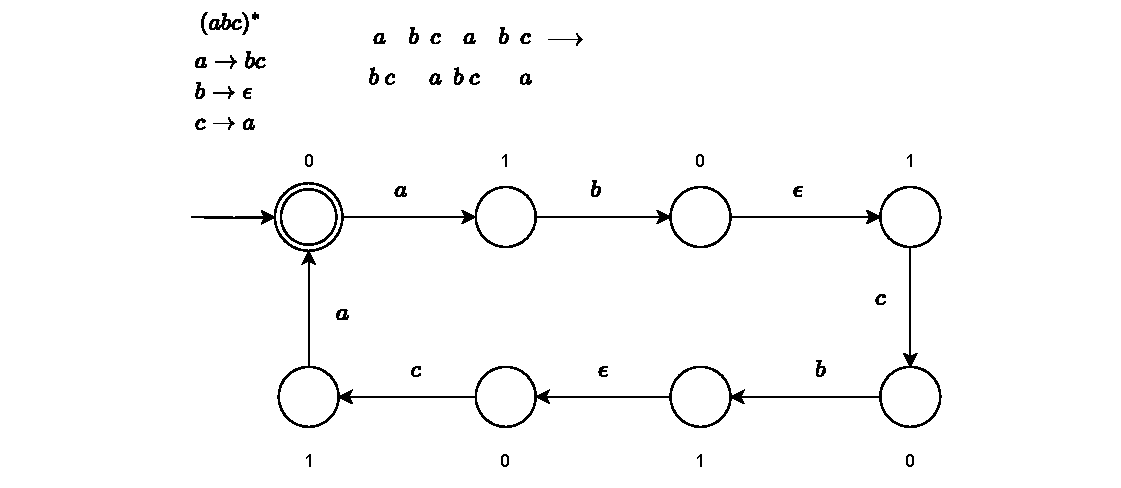
\includegraphics[scale=1.0,keepaspectratio]{obrazky-figures/transducer_in_mata.drawio.pdf}
    \caption{
      2-tape \nft from Example~\ref{example:2_tape_nft} represented in \mata as an \nfaClass with states annotated by state levels.
    }\label{fig:2_tape_nft_in_mata}
  \end{figure}
\end{example}

\subsection{No Operation Transitions}
An epsilon transition from a state with level $k$ to $k+1 \mod n$ can be understood as a \emph{no operation transition} \nop, i.e., a transition where the current tape does not perform any operation (no reading nor writing). In essence the impact of the transition is the same as if reading an empty string on the current tape.

In constrast, an epsilon transition from a state with level $k$ to another state with level $k$ is a simple change of states (as per the usual definition of epsilon transitions in \nfas).

Depending on the application, one might prefer to use one or the other representation as needed.
In this work, we use \nop when we want to explicitly stress the distinction between a simple change of state in \nft (an epsilon transition between states with the same level), and no operation on a current tape (tape does not read nor writes any symbol).

\section{Algorithms}
\label{sec:Algorithms}

\begin{itemize}
  \item Synchronization,
  \item intersection,
  \item composition,
  \item concatenate
  \item Application,
  \item Projection (to, out),
  \item get\_one\_letter\_aut
  \item \ldots
\end{itemize}

\subsection{Synchronization}

All operations performing some kind of traversal over the transitions start the compution from states with level $0$.
\nfts are always synchronized on states with level $0$, that is, after each \nft transition is completed (all tape operations are handled).
If the macro-state in a worklist contains only states of multiple \nfts with levels $0$, the \nfts are synchronized and the next macro-state can be computed.
When the synchronized \nfts perform one transition, due to the supported jumps, the new macro state may contain states with different levels.
Only the state in the macro-state with the level furthest behind is expanded.
The others are at least one step ahead and therefore cannot be expanded and must wait for the states behind to get to at least their levels first before being expanded themselves.

Since jumps can jump at most to the next state with level $0$, we always know which states in the macro-state are ahead and which are behind.
If we expand a macro-state with states with levels $k$ and $l$ where $k > l$, we know that state with level $k$ must be ahead of the state with level $l$.
If any of the states has level $0$ (and there are other states with nonzero levels), we know that the state $0$ must be ahead of all the other states with nonzero levels and synchronized with all other states with levels $0$ since the states with levels $0$ can only be the next states with levels $0$, and not the states with level $0$ behind.

The same holds for BDDs utilizing the same data structure and constraints as \nfts.

\begin{example}
  If we perform synchronization over three $4$-tape \nfts, starting from macro-state with levels $(0, 0, 0)$, we perform one transition and may end up in a macro-state with levels $(3, 1, 0)$ where the first \nft made a jump of length $3$, the second performed normal transition (jump of length $0$), and the last \nft performed a jump to the next state with level $0$.
  When expanding the macro-state $(3, 1, 0)$ later on, we know that the state with level $0$ is ahead of the other states with levels $3$ and $1$. And we further know that state with level $3$ must be ahead of the state with level $1$. Therefore, the state with level $1$ must be expanded up until the level reaches $3$ or greater (the next level $0$).
  Then we may get $(3, 3, 0)$, both the first and the second state are expanded to states with levels $(0, 0, 0)$ and the macro-state is synchronized again.
\end{example}

\begin{figure}[ht]
  \centering
  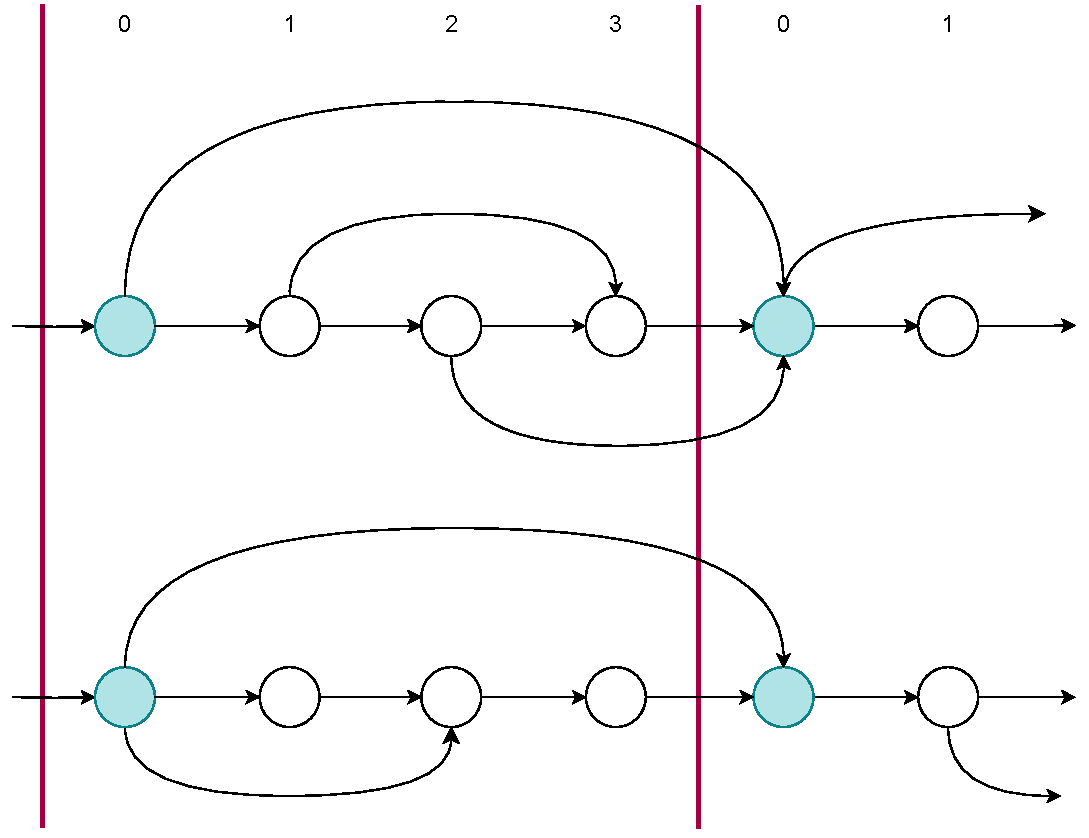
\includegraphics[scale=0.7, keepaspectratio]{obrazky-figures/jumps_synchronization.drawio.pdf}
  \caption{
    An example of allowed jumps in $4$-tape \nfts during synchronization.
    Jumps can start in state with any level and jump up to the next state with level $0$.
    The jumps cannot jump over states with level $0$, however.
  }

\end{figure}


\paragraph{Alternative representation of jumps.}
If the restriction of allowed jumps being only to the next state with level $0$ is too strict, an alternative approach where jumps are allowed to jump over (potentially multiple) states with level $0$ can be chosen.
However, during operations such as product construction, an additional information must be added to the worklist containing macro-states containing a list of lengths of each jump performed during the expansion of the last macro state in order to know how far ahead are the states jumped to in relation to the other states in the macro-state.

We deem this approach inferior to our chosen appraoch since it distorts the simplicity of a single data structure and algorithms on it for NFAs, \nfts, and BDDs.


% Basic approach, operations, representation
\section{Finite Transducers for String Solving}

TODO: Modelling replace operations

\subsection{Algorithms}
\begin{itemize}
  \item Reluctant replacement~\cite{replace_nfts_model_ModelingRegularReplacementForStringConstraintSolving_DBLP:conf/nfm/FuL10}
  \begin{itemize}
    \item \dfts for finite replacement
    \item \nfts for left-most reluctant replacement
    \item differences for single literal, single symbol, regular langauge
    \item differences for single replacement and all replacement
  \end{itemize}
\end{itemize}

\chapter{Implementation}

The proposed data structures for finite transducers, standard operations on finite transducers, and algorithms for modelling replace operations were implemented in \mata.

The majority of the operations on finite transducers closely follow the implementation of the corresponding operations on \nfas already existing in \mata.
These operations are modified only in places where it is necessary to handle the differences between \nfas and \nfts, such as correctly setting and resetting the vector of levels for transducer states, or handling epsilon, \nop and don't care symbols.

Furthermore, several algorithms specific for \nfts are added to \mata, namely composition of two \nfts, application (of both an \nfa and a word) on an \nft, projection (to a specified subset of \nft tapes---producing a new \nft---or to only a single tape---producing the corresponding \nfa for the specified tape).

\paragraph{Levels.}
The vector of levels is a vector of unsigned integers representin the levels indexed by states.

Each \nft also stores the number of tapes (levels) in the \nft.
The number of tapes defaults to $1$, which means that the \nft is equivalent to \nfa and the operations on \nfts with number of levels set to $1$ will behave the same as a corresponding \nfa (with an equivalent transition relation where all don't care transitions are replaced with transition between the same states over the whole alphabet).

This is useful as it keeps the data structures in \mata consitent with the behaviour expected by many potential users of \mata.

\paragraph{Epsilon and no operation transitions.}
We have decided to unify the symbols for epsilon transitions and \nop transitions used in \mata.
We represent both transitions with a transition over an epsilon symbol $\epsilon$, corresponding to the largest unsigned integer value of a symbol in \mata.

To distinguish between both, we check whether the epsilon transition leads from a state with level $k$ to a state with level $k + 1 \mod n$ or not whenever we encounter the symbol in algorithms.
This operation has constant complexity since a set of levels in \mata is a state-idexable vector of levels.

We decided for this approach since all operations in \mata already support epsilon transitions, checking for existence of epsilon transitions and accessing them has constant complexity, and adding handling for yet another special transition symbol is further complicates the logic for many operations which do not have to distinguish between epsilon and no operation transitions.

\paragraph{Words and identity insertion.}
We also implemented a few utility functions which are useful when constructing or modifying \nfts\footnote{Especially for modelling the replace and other operations in string solving.} such as
\begin{itemize}
  \item \emph{inserting an identity transition} over all tapes (all tapes read/write the same symbol) over the given alphabet for a specified state.

  This is specially useful for string solving where usually one specially handles a small subset of transitions symbols, but wants to leave the remaining symbols in the input word unmodified.

  \item \emph{inserting a word} for specified tapes or \emph{inserting words}, one for each tape.

  This allows one to quickly create transducers which read a specific word, replace a specific string literal with a given literal, or removes specified literal from the input word.
\end{itemize}


\chapter{Experimental Evaluation}

\chapter{Conclusion}

%=========================================================================

% For compilation piecewise (see projekt.tex), it is necessary to uncomment it
% \end{document}
